% Options for packages loaded elsewhere
\PassOptionsToPackage{unicode}{hyperref}
\PassOptionsToPackage{hyphens}{url}
%
\documentclass[
  12pt,
]{article}
\usepackage{amsmath,amssymb}
\usepackage{iftex}
\ifPDFTeX
  \usepackage[T1]{fontenc}
  \usepackage[utf8]{inputenc}
  \usepackage{textcomp} % provide euro and other symbols
\else % if luatex or xetex
  \usepackage{unicode-math} % this also loads fontspec
  \defaultfontfeatures{Scale=MatchLowercase}
  \defaultfontfeatures[\rmfamily]{Ligatures=TeX,Scale=1}
\fi
\usepackage{lmodern}
\ifPDFTeX\else
  % xetex/luatex font selection
    \setmainfont[]{Times New Roman}
\fi
% Use upquote if available, for straight quotes in verbatim environments
\IfFileExists{upquote.sty}{\usepackage{upquote}}{}
\IfFileExists{microtype.sty}{% use microtype if available
  \usepackage[]{microtype}
  \UseMicrotypeSet[protrusion]{basicmath} % disable protrusion for tt fonts
}{}
\makeatletter
\@ifundefined{KOMAClassName}{% if non-KOMA class
  \IfFileExists{parskip.sty}{%
    \usepackage{parskip}
  }{% else
    \setlength{\parindent}{0pt}
    \setlength{\parskip}{6pt plus 2pt minus 1pt}}
}{% if KOMA class
  \KOMAoptions{parskip=half}}
\makeatother
\usepackage{xcolor}
\usepackage[margin=1in]{geometry}
\usepackage{color}
\usepackage{fancyvrb}
\newcommand{\VerbBar}{|}
\newcommand{\VERB}{\Verb[commandchars=\\\{\}]}
\DefineVerbatimEnvironment{Highlighting}{Verbatim}{commandchars=\\\{\}}
% Add ',fontsize=\small' for more characters per line
\usepackage{framed}
\definecolor{shadecolor}{RGB}{248,248,248}
\newenvironment{Shaded}{\begin{snugshade}}{\end{snugshade}}
\newcommand{\AlertTok}[1]{\textcolor[rgb]{0.94,0.16,0.16}{#1}}
\newcommand{\AnnotationTok}[1]{\textcolor[rgb]{0.56,0.35,0.01}{\textbf{\textit{#1}}}}
\newcommand{\AttributeTok}[1]{\textcolor[rgb]{0.13,0.29,0.53}{#1}}
\newcommand{\BaseNTok}[1]{\textcolor[rgb]{0.00,0.00,0.81}{#1}}
\newcommand{\BuiltInTok}[1]{#1}
\newcommand{\CharTok}[1]{\textcolor[rgb]{0.31,0.60,0.02}{#1}}
\newcommand{\CommentTok}[1]{\textcolor[rgb]{0.56,0.35,0.01}{\textit{#1}}}
\newcommand{\CommentVarTok}[1]{\textcolor[rgb]{0.56,0.35,0.01}{\textbf{\textit{#1}}}}
\newcommand{\ConstantTok}[1]{\textcolor[rgb]{0.56,0.35,0.01}{#1}}
\newcommand{\ControlFlowTok}[1]{\textcolor[rgb]{0.13,0.29,0.53}{\textbf{#1}}}
\newcommand{\DataTypeTok}[1]{\textcolor[rgb]{0.13,0.29,0.53}{#1}}
\newcommand{\DecValTok}[1]{\textcolor[rgb]{0.00,0.00,0.81}{#1}}
\newcommand{\DocumentationTok}[1]{\textcolor[rgb]{0.56,0.35,0.01}{\textbf{\textit{#1}}}}
\newcommand{\ErrorTok}[1]{\textcolor[rgb]{0.64,0.00,0.00}{\textbf{#1}}}
\newcommand{\ExtensionTok}[1]{#1}
\newcommand{\FloatTok}[1]{\textcolor[rgb]{0.00,0.00,0.81}{#1}}
\newcommand{\FunctionTok}[1]{\textcolor[rgb]{0.13,0.29,0.53}{\textbf{#1}}}
\newcommand{\ImportTok}[1]{#1}
\newcommand{\InformationTok}[1]{\textcolor[rgb]{0.56,0.35,0.01}{\textbf{\textit{#1}}}}
\newcommand{\KeywordTok}[1]{\textcolor[rgb]{0.13,0.29,0.53}{\textbf{#1}}}
\newcommand{\NormalTok}[1]{#1}
\newcommand{\OperatorTok}[1]{\textcolor[rgb]{0.81,0.36,0.00}{\textbf{#1}}}
\newcommand{\OtherTok}[1]{\textcolor[rgb]{0.56,0.35,0.01}{#1}}
\newcommand{\PreprocessorTok}[1]{\textcolor[rgb]{0.56,0.35,0.01}{\textit{#1}}}
\newcommand{\RegionMarkerTok}[1]{#1}
\newcommand{\SpecialCharTok}[1]{\textcolor[rgb]{0.81,0.36,0.00}{\textbf{#1}}}
\newcommand{\SpecialStringTok}[1]{\textcolor[rgb]{0.31,0.60,0.02}{#1}}
\newcommand{\StringTok}[1]{\textcolor[rgb]{0.31,0.60,0.02}{#1}}
\newcommand{\VariableTok}[1]{\textcolor[rgb]{0.00,0.00,0.00}{#1}}
\newcommand{\VerbatimStringTok}[1]{\textcolor[rgb]{0.31,0.60,0.02}{#1}}
\newcommand{\WarningTok}[1]{\textcolor[rgb]{0.56,0.35,0.01}{\textbf{\textit{#1}}}}
\usepackage{longtable,booktabs,array}
\usepackage{calc} % for calculating minipage widths
% Correct order of tables after \paragraph or \subparagraph
\usepackage{etoolbox}
\makeatletter
\patchcmd\longtable{\par}{\if@noskipsec\mbox{}\fi\par}{}{}
\makeatother
% Allow footnotes in longtable head/foot
\IfFileExists{footnotehyper.sty}{\usepackage{footnotehyper}}{\usepackage{footnote}}
\makesavenoteenv{longtable}
\usepackage{graphicx}
\makeatletter
\def\maxwidth{\ifdim\Gin@nat@width>\linewidth\linewidth\else\Gin@nat@width\fi}
\def\maxheight{\ifdim\Gin@nat@height>\textheight\textheight\else\Gin@nat@height\fi}
\makeatother
% Scale images if necessary, so that they will not overflow the page
% margins by default, and it is still possible to overwrite the defaults
% using explicit options in \includegraphics[width, height, ...]{}
\setkeys{Gin}{width=\maxwidth,height=\maxheight,keepaspectratio}
% Set default figure placement to htbp
\makeatletter
\def\fps@figure{htbp}
\makeatother
\setlength{\emergencystretch}{3em} % prevent overfull lines
\providecommand{\tightlist}{%
  \setlength{\itemsep}{0pt}\setlength{\parskip}{0pt}}
\setcounter{secnumdepth}{5}
% definitions for citeproc citations
\NewDocumentCommand\citeproctext{}{}
\NewDocumentCommand\citeproc{mm}{%
  \begingroup\def\citeproctext{#2}\cite{#1}\endgroup}
\makeatletter
 % allow citations to break across lines
 \let\@cite@ofmt\@firstofone
 % avoid brackets around text for \cite:
 \def\@biblabel#1{}
 \def\@cite#1#2{{#1\if@tempswa , #2\fi}}
\makeatother
\newlength{\cslhangindent}
\setlength{\cslhangindent}{1.5em}
\newlength{\csllabelwidth}
\setlength{\csllabelwidth}{3em}
\newenvironment{CSLReferences}[2] % #1 hanging-indent, #2 entry-spacing
 {\begin{list}{}{%
  \setlength{\itemindent}{0pt}
  \setlength{\leftmargin}{0pt}
  \setlength{\parsep}{0pt}
  % turn on hanging indent if param 1 is 1
  \ifodd #1
   \setlength{\leftmargin}{\cslhangindent}
   \setlength{\itemindent}{-1\cslhangindent}
  \fi
  % set entry spacing
  \setlength{\itemsep}{#2\baselineskip}}}
 {\end{list}}
\usepackage{calc}
\newcommand{\CSLBlock}[1]{\hfill\break\parbox[t]{\linewidth}{\strut\ignorespaces#1\strut}}
\newcommand{\CSLLeftMargin}[1]{\parbox[t]{\csllabelwidth}{\strut#1\strut}}
\newcommand{\CSLRightInline}[1]{\parbox[t]{\linewidth - \csllabelwidth}{\strut#1\strut}}
\newcommand{\CSLIndent}[1]{\hspace{\cslhangindent}#1}
\usepackage{tcolorbox}
\usepackage{amssymb}
\usepackage{yfonts}
\usepackage{bm}
\usepackage{titlesec}
\usepackage{kbordermatrix}


\newtcolorbox{greybox}{
  colback=white,
  colframe=blue,
  coltext=black,
  boxsep=5pt,
  arc=4pt}
  
\newcommand{\sectionbreak}{\clearpage}

 
\newcommand{\ds}[4]{\sum_{{#1}=1}^{#3}\sum_{{#2}=1}^{#4}}
\newcommand{\us}[3]{\mathop{\sum\sum}_{1\leq{#2}<{#1}\leq{#3}}}

\newcommand{\ol}[1]{\overline{#1}}
\newcommand{\ul}[1]{\underline{#1}}

\newcommand{\amin}[1]{\mathop{\text{argmin}}_{#1}}
\newcommand{\amax}[1]{\mathop{\text{argmax}}_{#1}}

\newcommand{\ci}{\perp\!\!\!\perp}

\newcommand{\mc}[1]{\mathcal{#1}}
\newcommand{\mb}[1]{\mathbb{#1}}
\newcommand{\mf}[1]{\mathfrak{#1}}

\newcommand{\eps}{\epsilon}
\newcommand{\lbd}{\lambda}
\newcommand{\alp}{\alpha}
\newcommand{\df}{=:}
\newcommand{\am}[1]{\mathop{\text{argmin}}_{#1}}
\newcommand{\ls}[2]{\mathop{\sum\sum}_{#1}^{#2}}
\newcommand{\ijs}{\mathop{\sum\sum}_{1\leq i<j\leq n}}
\newcommand{\jis}{\mathop{\sum\sum}_{1\leq j<i\leq n}}
\newcommand{\sij}{\sum_{i=1}^n\sum_{j=1}^n}
	
\ifLuaTeX
  \usepackage{selnolig}  % disable illegal ligatures
\fi
\usepackage{bookmark}
\IfFileExists{xurl.sty}{\usepackage{xurl}}{} % add URL line breaks if available
\urlstyle{same}
\hypersetup{
  pdfauthor={Jan de Leeuw - University of California Los Angeles},
  hidelinks,
  pdfcreator={LaTeX via pandoc}}

\title{Smacof at 50: A Manual\\
Part x: Constrained Smacof}
\author{Jan de Leeuw - University of California Los Angeles}
\date{Started May 04, 2024, Version of May 04, 2024}

\begin{document}
\maketitle
\begin{abstract}
TBD
\end{abstract}

{
\setcounter{tocdepth}{3}
\tableofcontents
}
\textbf{Note:} This is a working manuscript which will be expanded/updated
frequently. All suggestions for improvement are welcome. All Rmd, tex,
html, pdf, R, and C files are in the public domain. Attribution will be
appreciated, but is not required. The various files can be found at
\url{https://github.com/deleeuw} in the repositories smacofCode, smacofManual,
and smacofExamples.

\section{Introduction}\label{introduction}

\section{General Theory}\label{general-theory}

De Leeuw and Heiser (1980)

\section{Linear Constraints}\label{linear-constraints}

\subsection{Subspace Constraints}\label{subspace-constraints}

\subsection{PQN Constraints}\label{pqn-constraints}

\[
Z:=\kbordermatrix{
\mbox{\ }&p&&q&&n\\
n&X&\mid&YA&\mid&D
}
\]

\section{Circular and Elliptical Constraints}\label{circular-and-elliptical-constraints}

De Leeuw (2007)
De Leeuw (2005)
De Leeuw and Mair (2009)
Minimize
\[
\omega(Y,\Lambda):=\text{tr}\ (\overline{X}-Y\Lambda)'V(\overline{X}-Y\Lambda)
\]
over diagonal \(\Lambda\) and \(Y\) with \(\text{diag}\ YY'=I\).

The optimal \(\Lambda\) for given \(Y\) is
\[
\Lambda = \text{diag}\ Y'V\overline{X} / \text{diag}\ Y'VY
\]

Let's look at all \(Y\) of the form \(Y=\tilde Y+e_i(y-\tilde y_i)'\). Then \(\omega\) is a function
of \(y\) and we can write
\[
\omega(y):=\omega(\tilde Y,\Lambda)+v_{ii}(y-\tilde y_i)'\Lambda^2(y-\tilde y_i)
-2e_i'V(X-\tilde Y\Lambda)\Lambda(y-\tilde y_i)
\]
Let \(H=V(X-\tilde Y\Lambda)\Lambda\). Then
\[
\omega(y)\leq\eta(y):=\omega(\tilde y_i)+v_{ii}\lambda_{\text{max}}^2(y-\tilde y_i)'(y-\tilde y_i)-2h_i'(y-\tilde y_i)
\]
Now suppose \(\hat y\) minimizes \(\eta\) over \(y'y=1\). Then
\[
\omega(\hat y)\leq\eta(\hat y)\leq\eta(\tilde y_i)=\omega(\tilde y_i)\
\]
Minimizing \(\eta\) over \(y'y=1\) can be done by maximizing
\[
y'\{\lambda_{\text{max}}^2v_{ii}\tilde y_i+h_i\}
\]
and thus \(\hat y\) is the term in \ldots{} curly brackets, normalized to unit length.

Let's check this in R. First generate some data.

\begin{Shaded}
\begin{Highlighting}[]
\CommentTok{\#set.seed(12345)}
\NormalTok{v }\OtherTok{\textless{}{-}} \SpecialCharTok{{-}}\FunctionTok{as.matrix}\NormalTok{(}\FunctionTok{dist}\NormalTok{(}\FunctionTok{matrix}\NormalTok{(}\FunctionTok{rnorm}\NormalTok{(}\DecValTok{12}\NormalTok{), }\DecValTok{6}\NormalTok{, }\DecValTok{2}\NormalTok{)))}
\FunctionTok{diag}\NormalTok{(v) }\OtherTok{\textless{}{-}} \SpecialCharTok{{-}}\FunctionTok{rowSums}\NormalTok{(v)}
\NormalTok{x }\OtherTok{\textless{}{-}} \FunctionTok{matrix}\NormalTok{(}\FunctionTok{rnorm}\NormalTok{(}\DecValTok{12}\NormalTok{),}\DecValTok{6}\NormalTok{,}\DecValTok{2}\NormalTok{)}
\NormalTok{x }\OtherTok{\textless{}{-}}\NormalTok{ v }\SpecialCharTok{\%*\%}\NormalTok{ x}
\NormalTok{y }\OtherTok{\textless{}{-}} \FunctionTok{matrix}\NormalTok{(}\FunctionTok{rnorm}\NormalTok{(}\DecValTok{12}\NormalTok{),}\DecValTok{6}\NormalTok{,}\DecValTok{2}\NormalTok{)}
\NormalTok{y }\OtherTok{\textless{}{-}}\NormalTok{ y }\SpecialCharTok{/} \FunctionTok{sqrt}\NormalTok{(}\FunctionTok{rowSums}\NormalTok{(y }\SpecialCharTok{\^{}} \DecValTok{2}\NormalTok{))}
\NormalTok{res }\OtherTok{\textless{}{-}}\NormalTok{ x }\SpecialCharTok{{-}}\NormalTok{ y}
\FunctionTok{print}\NormalTok{(}\FunctionTok{sum}\NormalTok{(res }\SpecialCharTok{*}\NormalTok{ (v }\SpecialCharTok{\%*\%}\NormalTok{ res)), }\AttributeTok{digits =} \DecValTok{10}\NormalTok{)}
\end{Highlighting}
\end{Shaded}

\begin{verbatim}
## [1] 42881.56515
\end{verbatim}

\begin{Shaded}
\begin{Highlighting}[]
\NormalTok{lbd }\OtherTok{\textless{}{-}} \FunctionTok{diag}\NormalTok{(}\FunctionTok{crossprod}\NormalTok{(y, v }\SpecialCharTok{\%*\%}\NormalTok{ x)) }\SpecialCharTok{/} \FunctionTok{diag}\NormalTok{(}\FunctionTok{crossprod}\NormalTok{(y, v }\SpecialCharTok{\%*\%}\NormalTok{ y))}
\NormalTok{mlbd }\OtherTok{\textless{}{-}} \FunctionTok{max}\NormalTok{(lbd }\SpecialCharTok{\^{}} \DecValTok{2}\NormalTok{)}
\NormalTok{lbd }\OtherTok{\textless{}{-}} \FunctionTok{diag}\NormalTok{(lbd)}
\NormalTok{res }\OtherTok{\textless{}{-}}\NormalTok{ x }\SpecialCharTok{{-}}\NormalTok{ y }\SpecialCharTok{\%*\%}\NormalTok{ lbd}
\FunctionTok{print}\NormalTok{(}\FunctionTok{sum}\NormalTok{(res }\SpecialCharTok{*}\NormalTok{ (v }\SpecialCharTok{\%*\%}\NormalTok{ res)), }\AttributeTok{digits =} \DecValTok{10}\NormalTok{)}
\end{Highlighting}
\end{Shaded}

\begin{verbatim}
## [1] 37269.35949
\end{verbatim}

Now change the first row of \(Y\).

\begin{Shaded}
\begin{Highlighting}[]
\NormalTok{h }\OtherTok{\textless{}{-}}\NormalTok{ v }\SpecialCharTok{\%*\%}\NormalTok{ res }\SpecialCharTok{\%*\%}\NormalTok{ lbd}
\NormalTok{g }\OtherTok{\textless{}{-}}\NormalTok{ mlbd }\SpecialCharTok{*}\NormalTok{ v[}\DecValTok{1}\NormalTok{, }\DecValTok{1}\NormalTok{] }\SpecialCharTok{*}\NormalTok{ y[}\DecValTok{1}\NormalTok{, ] }\SpecialCharTok{+}\NormalTok{ h[}\DecValTok{1}\NormalTok{, ]}
\NormalTok{y[}\DecValTok{1}\NormalTok{, ] }\OtherTok{\textless{}{-}}\NormalTok{ g }\SpecialCharTok{/} \FunctionTok{sqrt}\NormalTok{(}\FunctionTok{sum}\NormalTok{(g }\SpecialCharTok{\^{}} \DecValTok{2}\NormalTok{))}
\NormalTok{res }\OtherTok{\textless{}{-}}\NormalTok{ x }\SpecialCharTok{{-}}\NormalTok{ y }\SpecialCharTok{\%*\%}\NormalTok{ lbd}
\FunctionTok{print}\NormalTok{(}\FunctionTok{sum}\NormalTok{(res }\SpecialCharTok{*}\NormalTok{ (v }\SpecialCharTok{\%*\%}\NormalTok{ res)), }\AttributeTok{digits =} \DecValTok{10}\NormalTok{)}
\end{Highlighting}
\end{Shaded}

\begin{verbatim}
## [1] 37105.01009
\end{verbatim}

So far, so good. We can improve the first row again.

\begin{Shaded}
\begin{Highlighting}[]
\NormalTok{h }\OtherTok{\textless{}{-}}\NormalTok{ v }\SpecialCharTok{\%*\%}\NormalTok{ res }\SpecialCharTok{\%*\%}\NormalTok{ lbd}
\NormalTok{g }\OtherTok{\textless{}{-}}\NormalTok{ mlbd }\SpecialCharTok{*}\NormalTok{ v[}\DecValTok{1}\NormalTok{, }\DecValTok{1}\NormalTok{] }\SpecialCharTok{*}\NormalTok{ y[}\DecValTok{1}\NormalTok{, ] }\SpecialCharTok{+}\NormalTok{ h[}\DecValTok{1}\NormalTok{, ]}
\NormalTok{y[}\DecValTok{1}\NormalTok{, ] }\OtherTok{\textless{}{-}}\NormalTok{ g }\SpecialCharTok{/} \FunctionTok{sqrt}\NormalTok{(}\FunctionTok{sum}\NormalTok{(g }\SpecialCharTok{\^{}} \DecValTok{2}\NormalTok{))}
\NormalTok{res }\OtherTok{\textless{}{-}}\NormalTok{ x }\SpecialCharTok{{-}}\NormalTok{ y }\SpecialCharTok{\%*\%}\NormalTok{ lbd}
\FunctionTok{print}\NormalTok{(}\FunctionTok{sum}\NormalTok{(res }\SpecialCharTok{*}\NormalTok{ (v }\SpecialCharTok{\%*\%}\NormalTok{ res)), }\AttributeTok{digits =} \DecValTok{10}\NormalTok{)}
\end{Highlighting}
\end{Shaded}

\begin{verbatim}
## [1] 37085.35919
\end{verbatim}

Instead of continuing to iteratively improve the first row we'll make a loop over the rows of \(Y\).

\begin{Shaded}
\begin{Highlighting}[]
\ControlFlowTok{for}\NormalTok{ (i }\ControlFlowTok{in} \DecValTok{1}\SpecialCharTok{:}\DecValTok{6}\NormalTok{) \{}
\NormalTok{  h }\OtherTok{\textless{}{-}}\NormalTok{ v }\SpecialCharTok{\%*\%}\NormalTok{ res }\SpecialCharTok{\%*\%}\NormalTok{ lbd}
\NormalTok{  g }\OtherTok{\textless{}{-}}\NormalTok{ mlbd }\SpecialCharTok{*}\NormalTok{ v[i, i] }\SpecialCharTok{*}\NormalTok{ y[i,] }\SpecialCharTok{+}\NormalTok{ h[i,]}
\NormalTok{  y[i,] }\OtherTok{\textless{}{-}}\NormalTok{ g }\SpecialCharTok{/} \FunctionTok{sqrt}\NormalTok{(}\FunctionTok{sum}\NormalTok{(g }\SpecialCharTok{\^{}} \DecValTok{2}\NormalTok{))}
\NormalTok{  res }\OtherTok{\textless{}{-}}\NormalTok{ x }\SpecialCharTok{{-}}\NormalTok{ y }\SpecialCharTok{\%*\%}\NormalTok{ lbd}
  \FunctionTok{print}\NormalTok{(}\FunctionTok{sum}\NormalTok{(res }\SpecialCharTok{*}\NormalTok{ (v }\SpecialCharTok{\%*\%}\NormalTok{ res)), }\AttributeTok{digits =} \DecValTok{10}\NormalTok{)}
\NormalTok{\}}
\end{Highlighting}
\end{Shaded}

\begin{verbatim}
## [1] 37081.1818
## [1] 32673.02149
## [1] 30777.27021
## [1] 30754.50963
## [1] 29558.44564
## [1] 29392.35169
\end{verbatim}

We can do this again.

\begin{Shaded}
\begin{Highlighting}[]
\ControlFlowTok{for}\NormalTok{ (i }\ControlFlowTok{in} \DecValTok{1}\SpecialCharTok{:}\DecValTok{6}\NormalTok{) \{}
\NormalTok{  h }\OtherTok{\textless{}{-}}\NormalTok{ v }\SpecialCharTok{\%*\%}\NormalTok{ res }\SpecialCharTok{\%*\%}\NormalTok{ lbd}
\NormalTok{  g }\OtherTok{\textless{}{-}}\NormalTok{ mlbd }\SpecialCharTok{*}\NormalTok{ v[i, i] }\SpecialCharTok{*}\NormalTok{ y[i,] }\SpecialCharTok{+}\NormalTok{ h[i,]}
\NormalTok{  y[i,] }\OtherTok{\textless{}{-}}\NormalTok{ g }\SpecialCharTok{/} \FunctionTok{sqrt}\NormalTok{(}\FunctionTok{sum}\NormalTok{(g }\SpecialCharTok{\^{}} \DecValTok{2}\NormalTok{))}
\NormalTok{  res }\OtherTok{\textless{}{-}}\NormalTok{ x }\SpecialCharTok{{-}}\NormalTok{ y }\SpecialCharTok{\%*\%}\NormalTok{ lbd}
  \FunctionTok{print}\NormalTok{(}\FunctionTok{sum}\NormalTok{(res }\SpecialCharTok{*}\NormalTok{ (v }\SpecialCharTok{\%*\%}\NormalTok{ res)), }\AttributeTok{digits =} \DecValTok{10}\NormalTok{)}
\NormalTok{\}}
\end{Highlighting}
\end{Shaded}

\begin{verbatim}
## [1] 29320.30176
## [1] 26668.29102
## [1] 24209.88627
## [1] 24101.5816
## [1] 24097.29437
## [1] 24085.41324
\end{verbatim}

And again.

\begin{Shaded}
\begin{Highlighting}[]
\ControlFlowTok{for}\NormalTok{ (i }\ControlFlowTok{in} \DecValTok{1}\SpecialCharTok{:}\DecValTok{6}\NormalTok{) \{}
\NormalTok{  h }\OtherTok{\textless{}{-}}\NormalTok{ v }\SpecialCharTok{\%*\%}\NormalTok{ res }\SpecialCharTok{\%*\%}\NormalTok{ lbd}
\NormalTok{  g }\OtherTok{\textless{}{-}}\NormalTok{ mlbd }\SpecialCharTok{*}\NormalTok{ v[i, i] }\SpecialCharTok{*}\NormalTok{ y[i,] }\SpecialCharTok{+}\NormalTok{ h[i,]}
\NormalTok{  y[i,] }\OtherTok{\textless{}{-}}\NormalTok{ g }\SpecialCharTok{/} \FunctionTok{sqrt}\NormalTok{(}\FunctionTok{sum}\NormalTok{(g }\SpecialCharTok{\^{}} \DecValTok{2}\NormalTok{))}
\NormalTok{  res }\OtherTok{\textless{}{-}}\NormalTok{ x }\SpecialCharTok{{-}}\NormalTok{ y }\SpecialCharTok{\%*\%}\NormalTok{ lbd}
  \FunctionTok{print}\NormalTok{(}\FunctionTok{sum}\NormalTok{(res }\SpecialCharTok{*}\NormalTok{ (v }\SpecialCharTok{\%*\%}\NormalTok{ res)), }\AttributeTok{digits =} \DecValTok{10}\NormalTok{)}
\NormalTok{\}}
\end{Highlighting}
\end{Shaded}

\begin{verbatim}
## [1] 24081.3095
## [1] 23998.12667
## [1] 23153.05054
## [1] 23103.02434
## [1] 23083.08752
## [1] 23037.69143
\end{verbatim}

These are still for the same \(\Lambda\). We can compute a new \(\Lambda\).

\begin{Shaded}
\begin{Highlighting}[]
\NormalTok{lbd }\OtherTok{\textless{}{-}} \FunctionTok{diag}\NormalTok{(}\FunctionTok{crossprod}\NormalTok{(y, v }\SpecialCharTok{\%*\%}\NormalTok{ x)) }\SpecialCharTok{/} \FunctionTok{diag}\NormalTok{(}\FunctionTok{crossprod}\NormalTok{(y, v }\SpecialCharTok{\%*\%}\NormalTok{ y))}
\NormalTok{mlbd }\OtherTok{\textless{}{-}} \FunctionTok{max}\NormalTok{(lbd }\SpecialCharTok{\^{}} \DecValTok{2}\NormalTok{)}
\NormalTok{lbd }\OtherTok{\textless{}{-}} \FunctionTok{diag}\NormalTok{(lbd)}
\NormalTok{res }\OtherTok{\textless{}{-}}\NormalTok{ x }\SpecialCharTok{{-}}\NormalTok{ y }\SpecialCharTok{\%*\%}\NormalTok{ lbd}
\FunctionTok{print}\NormalTok{(}\FunctionTok{sum}\NormalTok{(res }\SpecialCharTok{*}\NormalTok{ (v }\SpecialCharTok{\%*\%}\NormalTok{ res)), }\AttributeTok{digits =} \DecValTok{10}\NormalTok{)}
\end{Highlighting}
\end{Shaded}

\begin{verbatim}
## [1] 4731.567776
\end{verbatim}

And then start updating \(Y\) again.

\begin{Shaded}
\begin{Highlighting}[]
\ControlFlowTok{for}\NormalTok{ (i }\ControlFlowTok{in} \DecValTok{1}\SpecialCharTok{:}\DecValTok{6}\NormalTok{) \{}
\NormalTok{  h }\OtherTok{\textless{}{-}}\NormalTok{ v }\SpecialCharTok{\%*\%}\NormalTok{ res }\SpecialCharTok{\%*\%}\NormalTok{ lbd}
\NormalTok{  g }\OtherTok{\textless{}{-}}\NormalTok{ mlbd }\SpecialCharTok{*}\NormalTok{ v[i, i] }\SpecialCharTok{*}\NormalTok{ y[i,] }\SpecialCharTok{+}\NormalTok{ h[i,]}
\NormalTok{  y[i,] }\OtherTok{\textless{}{-}}\NormalTok{ g }\SpecialCharTok{/} \FunctionTok{sqrt}\NormalTok{(}\FunctionTok{sum}\NormalTok{(g }\SpecialCharTok{\^{}} \DecValTok{2}\NormalTok{))}
\NormalTok{  res }\OtherTok{\textless{}{-}}\NormalTok{ x }\SpecialCharTok{{-}}\NormalTok{ y }\SpecialCharTok{\%*\%}\NormalTok{ lbd}
  \FunctionTok{print}\NormalTok{(}\FunctionTok{sum}\NormalTok{(res }\SpecialCharTok{*}\NormalTok{ (v }\SpecialCharTok{\%*\%}\NormalTok{ res)), }\AttributeTok{digits =} \DecValTok{10}\NormalTok{)}
\NormalTok{\}}
\end{Highlighting}
\end{Shaded}

\begin{verbatim}
## [1] 4546.999526
## [1] 4438.990353
## [1] 4378.626778
## [1] 4239.591729
## [1] 3779.169994
## [1] 2072.594059
\end{verbatim}

And so on. Let's look at the result so far. The blue points are \(X\), the red points are \(Y\),
on an ellips with centered at the origin with the coordinate axes as minor and major axes.

\begin{Shaded}
\begin{Highlighting}[]
\FunctionTok{par}\NormalTok{(}\AttributeTok{pty =} \StringTok{"s"}\NormalTok{)}
\NormalTok{z }\OtherTok{\textless{}{-}}\NormalTok{ y }\SpecialCharTok{\%*\%}\NormalTok{ lbd}
\FunctionTok{plot}\NormalTok{(}\FunctionTok{rbind}\NormalTok{(x, z), }\AttributeTok{type =} \StringTok{"n"}\NormalTok{, }\AttributeTok{xlab =} \StringTok{"dimension 1"}\NormalTok{, }\AttributeTok{ylab =} \StringTok{"dimension 2"}\NormalTok{)}
\FunctionTok{points}\NormalTok{(x, }\AttributeTok{col =} \StringTok{"BLUE"}\NormalTok{, }\AttributeTok{pch =} \DecValTok{16}\NormalTok{)}
\FunctionTok{points}\NormalTok{(z, }\AttributeTok{col =} \StringTok{"RED"}\NormalTok{, }\AttributeTok{pch =} \DecValTok{16}\NormalTok{)}
\FunctionTok{abline}\NormalTok{(}\AttributeTok{v =} \DecValTok{0}\NormalTok{)}
\FunctionTok{abline}\NormalTok{(}\AttributeTok{h =} \DecValTok{0}\NormalTok{)}
\ControlFlowTok{for}\NormalTok{ (i }\ControlFlowTok{in} \DecValTok{1}\SpecialCharTok{:}\DecValTok{6}\NormalTok{) \{}
  \FunctionTok{lines}\NormalTok{(}\FunctionTok{matrix}\NormalTok{(}\FunctionTok{c}\NormalTok{(x[i, ], z[i, ]), }\DecValTok{2}\NormalTok{, }\DecValTok{2}\NormalTok{, }\AttributeTok{byrow =} \ConstantTok{TRUE}\NormalTok{))}
\NormalTok{\}}
\NormalTok{sc }\OtherTok{\textless{}{-}} \FunctionTok{seq}\NormalTok{(}\SpecialCharTok{{-}}\DecValTok{2} \SpecialCharTok{*}\NormalTok{ pi, }\DecValTok{2} \SpecialCharTok{*}\NormalTok{ pi, }\AttributeTok{length =} \DecValTok{100}\NormalTok{)}
\NormalTok{xc }\OtherTok{\textless{}{-}} \FunctionTok{cbind}\NormalTok{(}\FunctionTok{sin}\NormalTok{(sc), }\FunctionTok{cos}\NormalTok{(sc)) }\SpecialCharTok{\%*\%}\NormalTok{ lbd}
\FunctionTok{lines}\NormalTok{(xc, }\AttributeTok{col =} \StringTok{"RED"}\NormalTok{)}
\end{Highlighting}
\end{Shaded}

\begin{center}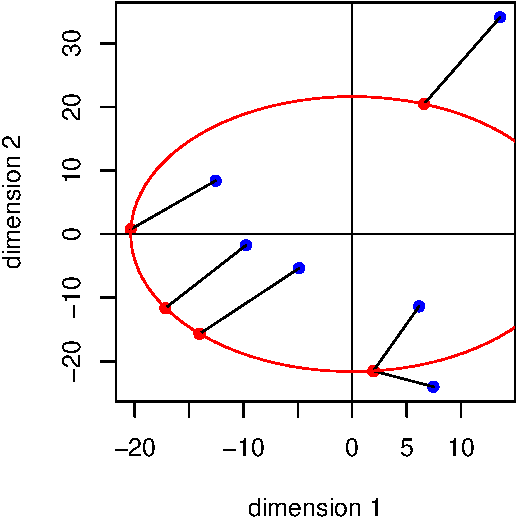
\includegraphics{smacofCS_files/figure-latex/ploplo-1} \end{center}

Note that we have three nested infinite iterative processes here.

\begin{enumerate}
\def\labelenumi{\arabic{enumi}.}
\tightlist
\item
  Alternating the updates of \(\Lambda\) and \(Y\).
\item
  Cycling through the rows of \(Y\).
\item
  Updating a single row of \(Y\).
\end{enumerate}

We could reduce this to two processes by not using majorization in process 3
but computing the exact update of a row. Go back to
\[
\omega(y):=\omega(\tilde Y,\Lambda)+v_{ii}(y-\tilde y_i)'\Lambda^2(y-\tilde y_i)
-2h_i'(y-\tilde y_i)
\]
Minimizing \(\omega\) over \(y'y=1\) leads to the stationary equations
\[
(\Lambda^2-\mu I)y=g_i
\]
with
\[
g_i:=\frac{v_{ii}\Lambda^2\tilde y_i+h_i}{v_{ii}}
\]
and \(\mu\) a Lagrange multiplier. This is one of the famous secular equations (see for instance Hager (2001)), which can be solved by finding a root of the equation
\[
\phi(\mu):=\sum_{s=1}^p\frac{g_{is}^2}{(\lambda_s^2-\mu)^2}=1
\]
Also, of course, if we are fitting a circle then \(\Lambda\) is fixed at the identity and
matters simplify accordingly. Alternating the updates for \(\Lambda\) and \(Y\) is no longer
necessary.

\section*{References}\label{references}
\addcontentsline{toc}{section}{References}

\phantomsection\label{refs}
\begin{CSLReferences}{1}{0}
\bibitem[\citeproctext]{ref-deleeuw_U_05j}
De Leeuw, J. 2005. {``{Fitting Ellipsoids by Least Squares}.''} UCLA Department of Statistics. 2005. \url{https://jansweb.netlify.app/publication/deleeuw-u-05-j/deleeuw-u-05-j.pdf}.

\bibitem[\citeproctext]{ref-deleeuw_U_07h}
---------. 2007. {``{Quadratic Surface Embedding}.''} UCLA Department of Statistics. 2007. \url{https://jansweb.netlify.app/publication/deleeuw-u-07-h/deleeuw-u-07-h.pdf}.

\bibitem[\citeproctext]{ref-deleeuw_heiser_C_80}
De Leeuw, J., and W. J. Heiser. 1980. {``Multidimensional Scaling with Restrictions on the Configuration.''} In \emph{Multivariate Analysis, Volume {V}}, edited by P. R. Krishnaiah, 501--22. Amsterdam, The Netherlands: North Holland Publishing Company.

\bibitem[\citeproctext]{ref-deleeuw_mair_A_09c}
De Leeuw, J., and P. Mair. 2009. {``{Multidimensional Scaling Using Majorization: SMACOF in R}.''} \emph{Journal of Statistical Software} 31 (3): 1--30. \url{https://www.jstatsoft.org/article/view/v031i03}.

\bibitem[\citeproctext]{ref-hager_01}
Hager, William W. 2001. {``{Minimizing a Quadratic over a Sphere}.''} \emph{SIAM Journal on Optimization} 12: 188--208.

\end{CSLReferences}

\end{document}
